\newpage

\section{Распределение предметных БД по узлам сети}

Согласно ТЗ, необходимо распределить предметные БД по узлам сети без учёта репликации. В настоящем документе приведены результаты вычислений, которые осуществлялись посредством электронных таблиц MS Excel. Соответствующие документы находятся в приложении.\par\bigskip

Необходимо определить вариант рационального размещения предметных баз данных в распределенной информационной системе для случая, когда каждая база данных размещается только в одном узле сети, а обрабатывающие процессы (приложения) не являются распределенными. При этом следует считать, что если некоторый процесс обращается за данными к базе, находящейся в другом узле, сетевые затраты на одно обращение составляют $t$ секунд, независимо от местонахождения узла в сети и дисциплины обслуживания. Если процесс обращается к базе данных, находящейся в том же узле, где выполняется процесс, то следует считать, что $t = 0$.

Таблица~\ref{table:db_usage} показывает использование предметных баз данных обрабатывающими процессами (приложениями) в течение временного интервала и интенсивности их обращений к базам данных (среднее число обращений за рассматриваемый интервал времени).

\begin{table}[h]
\caption{Использование предметных баз данных}
\label{table:db_usage}
 \begin{tabular}{c}
 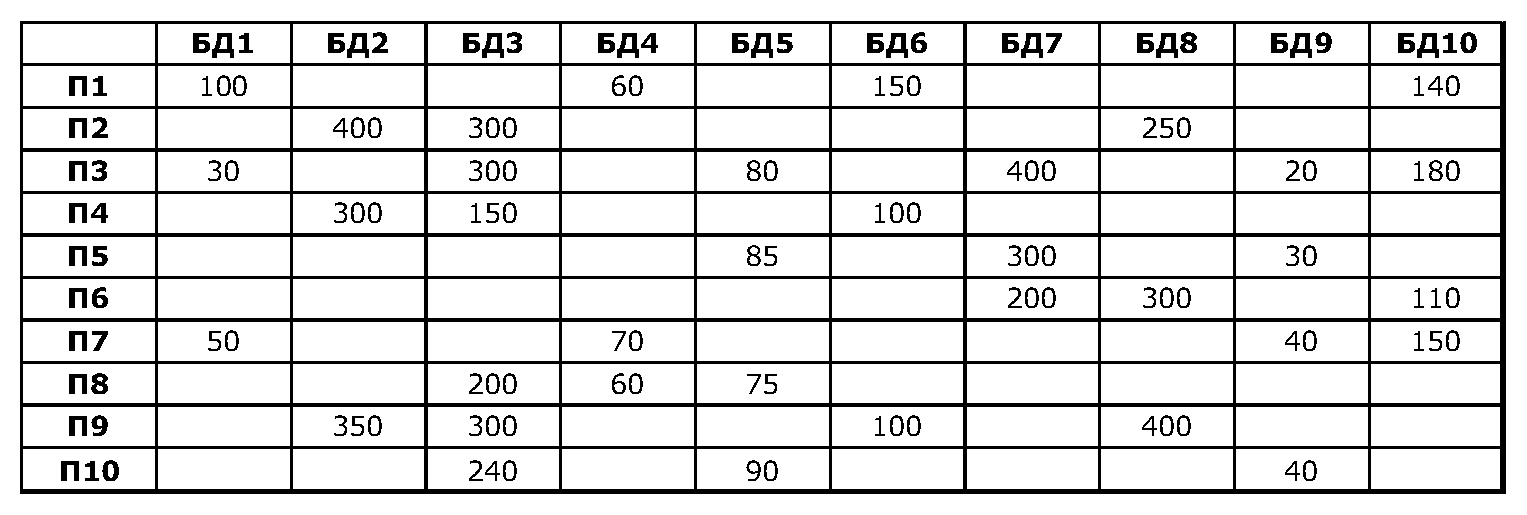
\includegraphics[width=1\linewidth]{pics/pic8_1_db_usage.eps}
 \end{tabular}
\end{table}

\newpage

Таблица~\ref{table:proc_distrib} показывает распределение обрабатывающих процессов по узлам распределённой сети.

\begin{table}[h]
\caption{Распределение обрабатывающих процессов по узлам}
\label{table:proc_distrib}
 \begin{tabular}{c}
 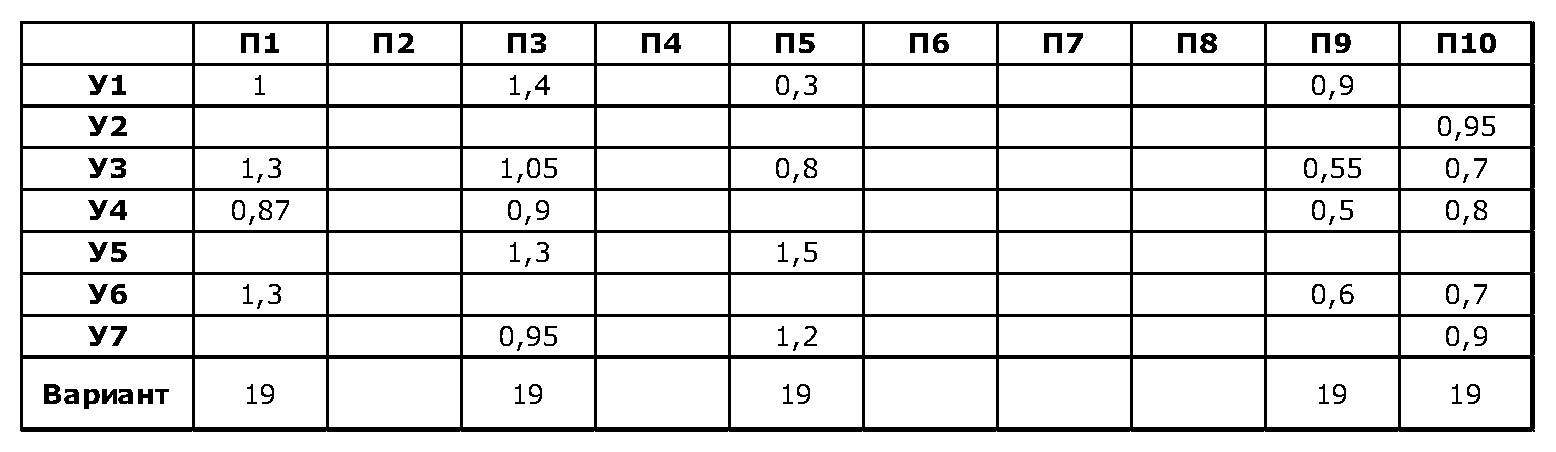
\includegraphics[width=1\linewidth]{pics/pic8_2_proc_disrib.eps}
 \end{tabular}
\end{table}

Коэффициенты в таблице~\ref{table:proc_distrib} используются для получения количества обращений к базе данных в исходном варианте задания по формуле:

$$N_1 = N\cdot k$$
где:\\
$N$ -– значение из таблицы~\ref{table:db_usage};\\
$k$ –- значение коэффициента из таблицы~\ref{table:proc_distrib};\\
$N_1$ -- результирующее значение для таблицы учебного варианта задания.\par\bigskip

\newpage

На основании данных из таблицы~\ref{table:db_usage} и таблицы~\ref{table:proc_distrib} для исходного варианта была сформирована сводная таблица исходных данных -- таблица~\ref{table:results}. Каждое значение этой таблицы есть среднее количество обращений к базе данных (БД$_i$) определенного процесса (П$_j$) из определенного узла сети (У$_k$).

\begin{table}[h]
\caption{Результаты затрат на обработку конкретной БД конкретными процессами в конкретных устройствах без учёта репликации}
\label{table:results}
 \begin{tabular}{c}
 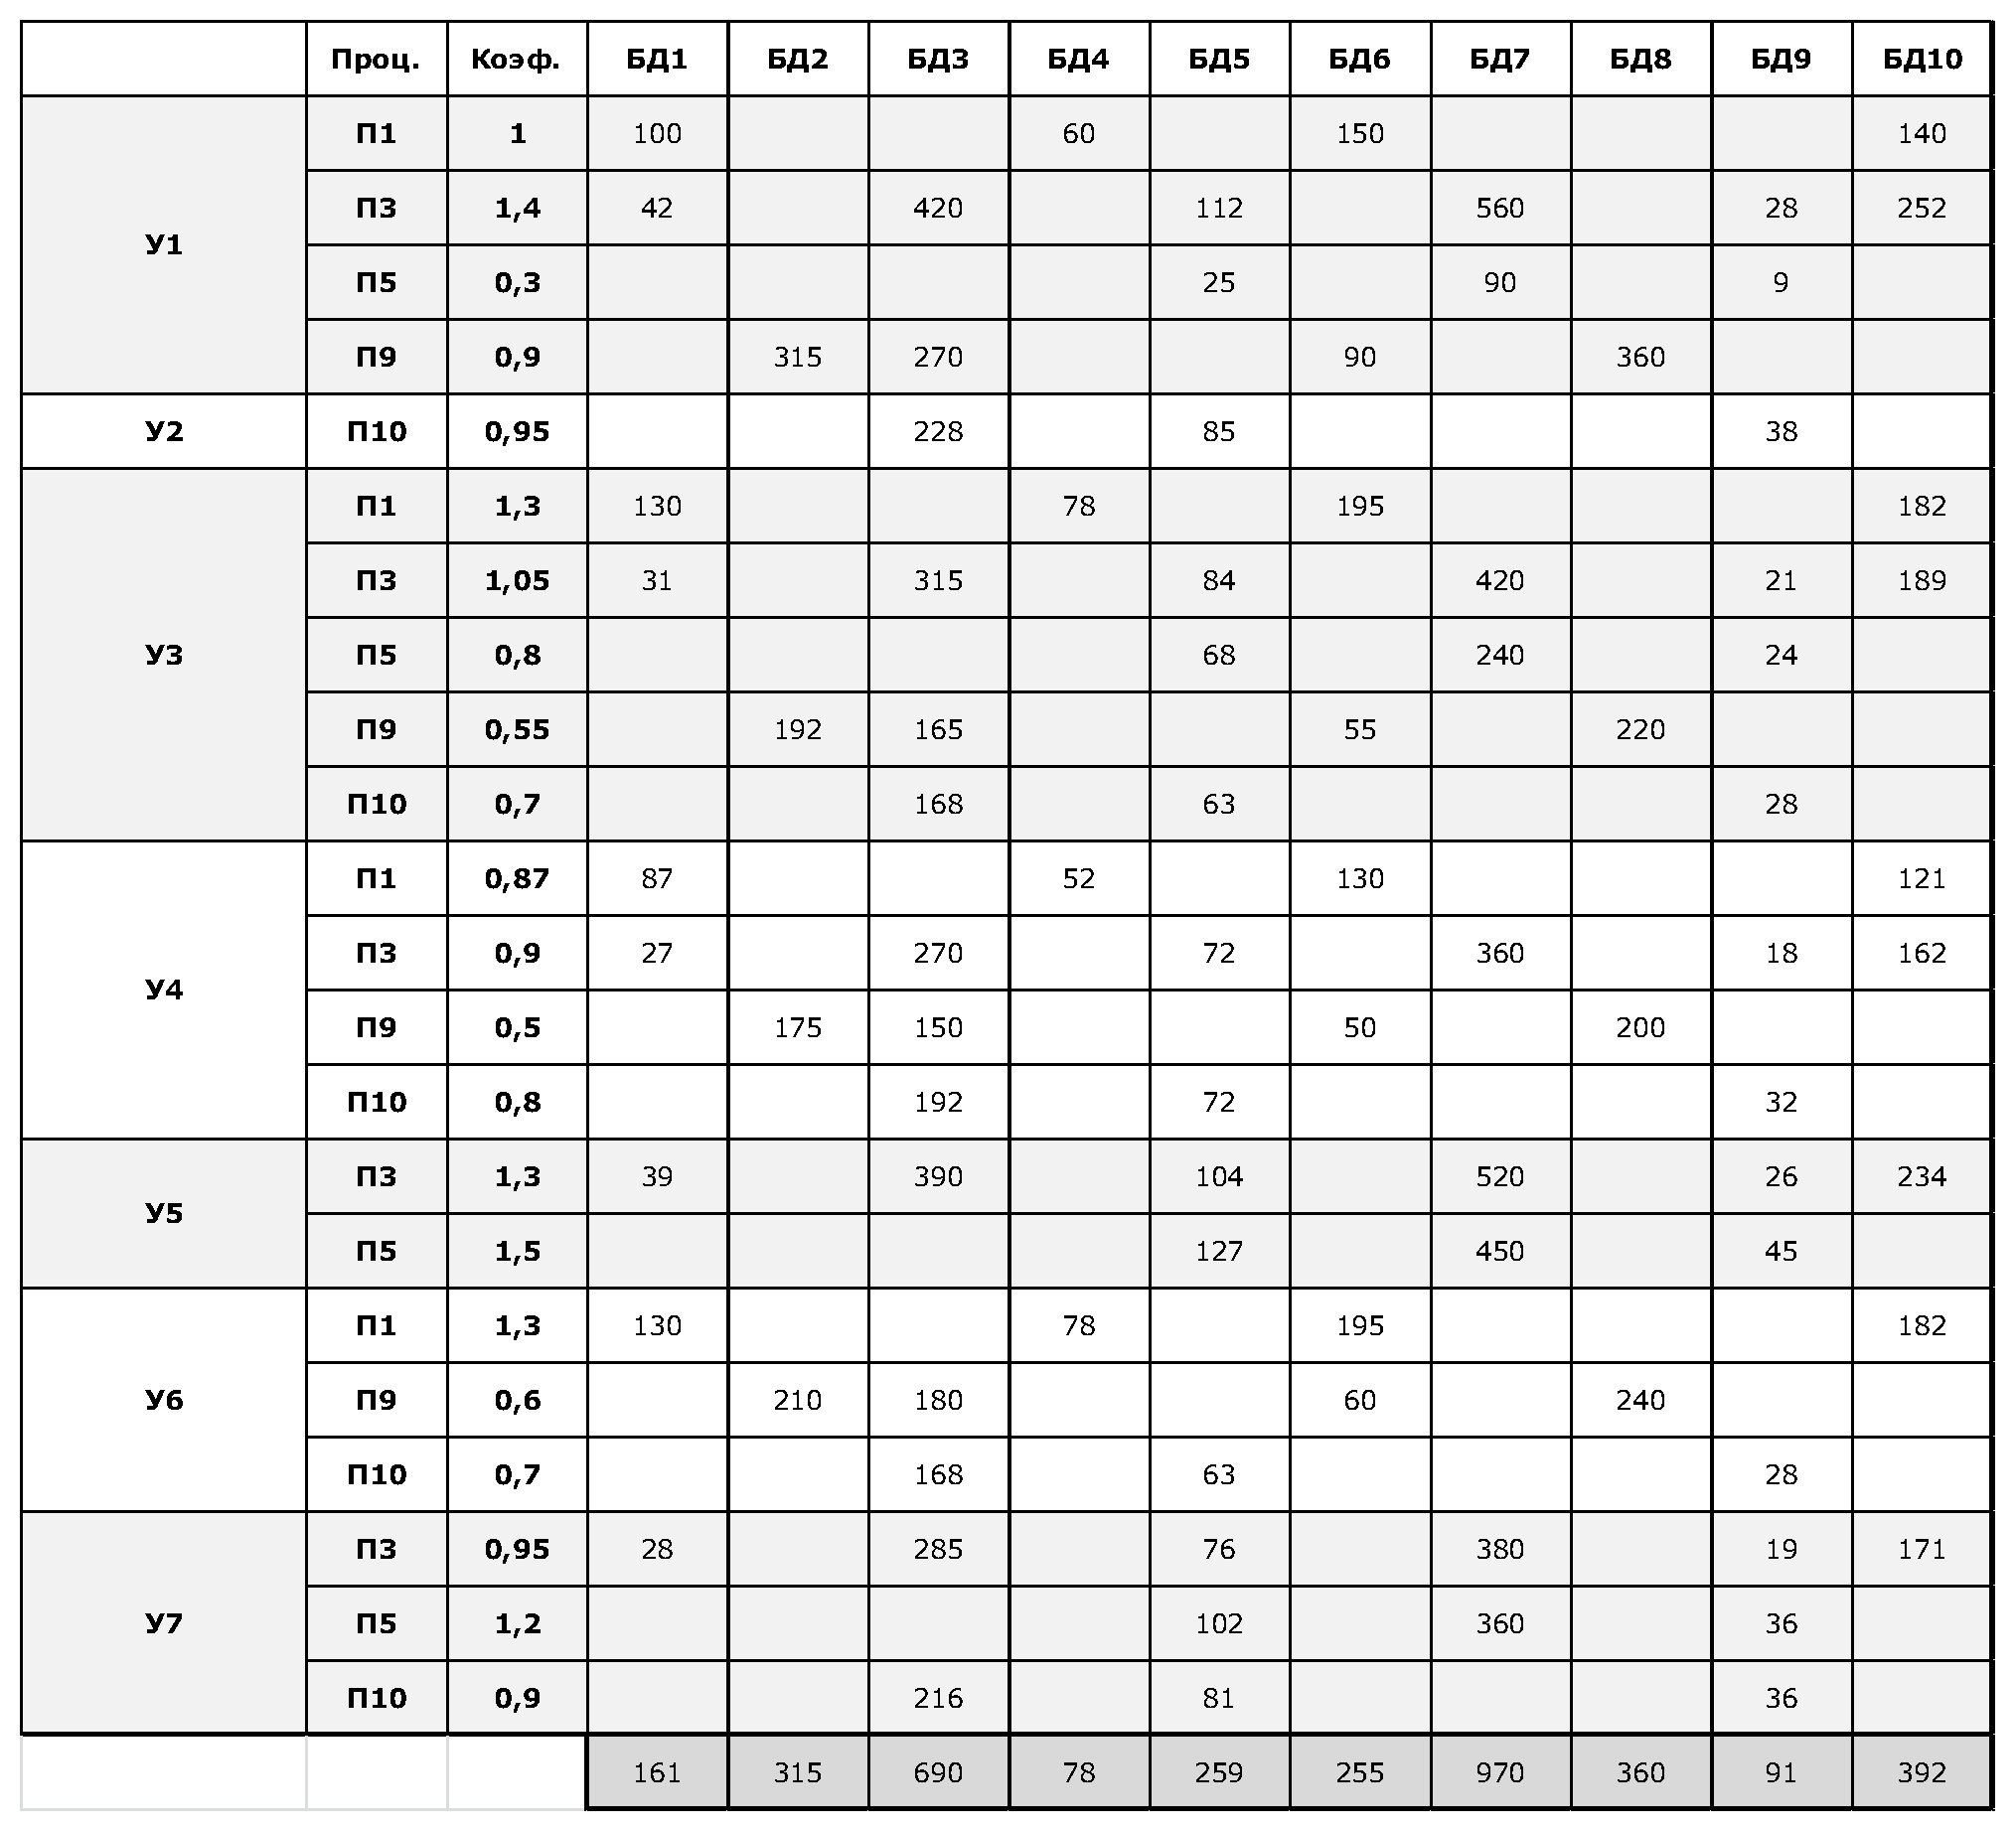
\includegraphics[width=1\linewidth]{pics/pic8_3_results.eps}
 \end{tabular}
\end{table}

\newpage

Составляем таблицу~\ref{table:sum_req}, в которой указываем все возможные варианты размещения баз данных по узлам сети. В каждую клетку этой таблицы записываем число, которое определяет суммарное количество всех запросов от всех процессов всех узлов к данной БД, при условии, что эта БД находится в данном узле.

\begin{table}[h]
\caption{Суммарное количество обращений к БД при возможных вариантах их размещения по узлам сети}
\label{table:sum_req}
 \begin{tabular}{c}
 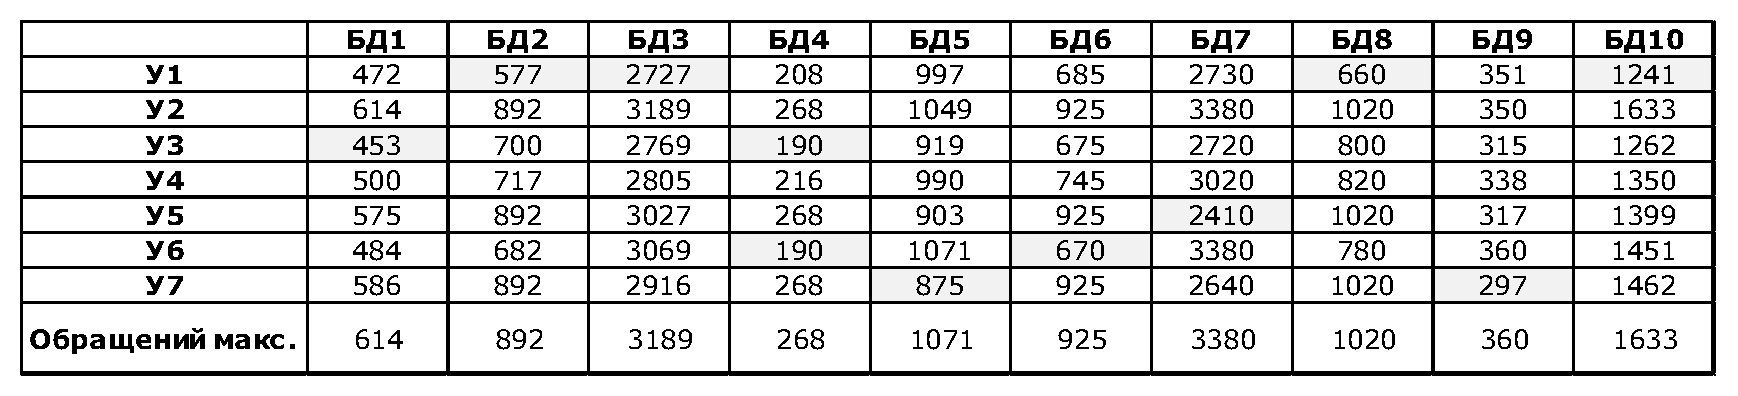
\includegraphics[width=1\linewidth]{pics/pic8_4_sum_req.eps}
 \end{tabular}
\end{table}

Используем правило: "Базу данных помещаем в тот узел, где она максимально используется, то есть суммарное количество обращений к ней со стороны других узлов минимально". Поэтому в каждом столбце, соответствующем одной конкретной БД, отыскиваем наименьшее значение. Это и будет соответствовать оптимальному варианту размещения этой БД, поскольку чем меньше это значение, тем меньше суммарное количество обращений от всех процессов всех других узлов к данной БД.\par\bigskip

Полученные результаты, показывающие оптимальные варианты размещения БД по узлам сети, записываем в таблицу~\ref{table:optimum}.

\begin{table}[h]
\caption{Оптимальные варианты размещения БД по узлам сети}
\label{table:optimum}
 \begin{tabular}{c}
 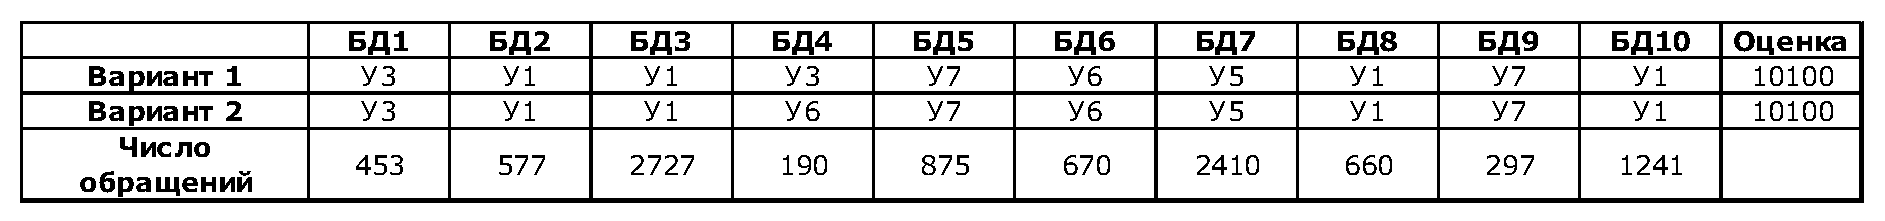
\includegraphics[width=1\linewidth]{pics/pic8_5_optimum.eps}
 \end{tabular}
\end{table}

Итак, получили, что в каждом из двух оптимальных вариантов размещения БД по узлам сети суммарное количество обращений ко всем БД, то есть суммарные затраты, составляет 10100.